\begin{frame}
\frametitle{Внешние устройства}
\begin{itemize}
  \item Допустим у вас есть сетевая карта:
  \begin{itemize}
    \item можно передать сетевой карте набор байт для отправки;
    \item сетевая карта может получать данные, процессор должен скопировать эти
    данные в память, обработать и "показать" пользователю;
    \item пакеты могут приходить в произвольные моменты времени.
  \end{itemize}
  \item Как узнать, что данные пришли на сетевую карту?
  \begin{itemize}
    \item можно спросить устройство (проверить какой-нибудь бит в каком-нибудь
    регистре устройства);
    \item такой вариант называют \emph{polling};
    \item пока код исполняемый процессором опрашивает устройство, процессор не
    делает ничего полезного.
  \end{itemize}
\end{itemize}
\end{frame}

\begin{frame}
\frametitle{Прерывания}
\begin{itemize}
  \item Прерывания - сигнал процессору, который "прерывает" текущий исполняемый
  код процессора
  \begin{itemize}
    \item сетевая карта посылает сигнал при получении данных;
    \item вместо исполняемого кода вызывается специальный обработчик прерывания;
    \item обработчик прерывания обслуживает устройство, и возвращает управление
    прерванному коду.
  \end{itemize}
  \item Следствия:
  \begin{itemize}
    \item не нужно тратить ресурсы процессора на бесполезный опрос устройств;
    \item прерванный код может быть не готов к тому, что его прервут - задача
    обработчика позаботится об этом.
  \end{itemize}
\end{itemize}
\end{frame}

\begin{frame}
\frametitle{Контроллер прерываний}
\begin{itemize}
  \item А что если у нас много устройств требующих внимания процессора?
  \begin{itemize}
    \item какое из устройств сгенерировало прерывание?
    \item если сразу несколько устройств сгенерировали прерывания?
  \end{itemize}
  \item Для разрешения этих проблем нужен посредник между устройствами и
  процессором
  \begin{itemize}
    \item такого посрденика называют контроллером прерываний;
    \item контроллер прерываний выполняет арбитраж.
  \end{itemize}
\end{itemize}
\end{frame}

\begin{frame}
\frametitle{Intel 8259}
\begin{columns}
  \begin{column}{0.7\textwidth}
  Intel 8259 - \emph{программируемый} контроллер прерываний (далее просто PIC)
  \begin{itemize}
    \item каскад из двух PIC использовался в IBM PC начиная с AT;
    \item сейчас он не используется, но его поведение эмулируется современными
    контроллерами прерываний.
  \end{itemize}
  \end{column}
  \begin{column}{0.3\textwidth}
    \begin{center}
      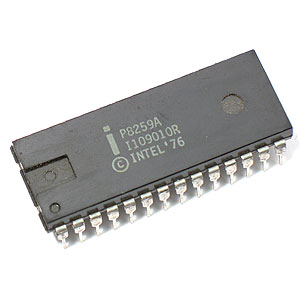
\includegraphics[width=\textwidth]{i8259.jpg}
    \end{center}
  \end{column}
\end{columns}
\end{frame}

\begin{frame}
\frametitle{Каскад intel 8259}
\begin{columns}
  \begin{column}{0.5\textwidth}
  \begin{center}
    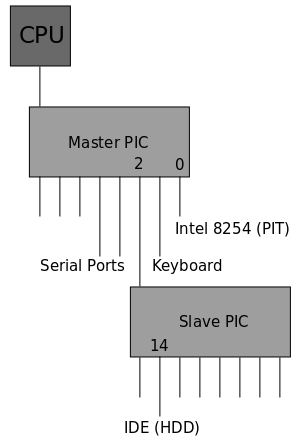
\includegraphics[height=0.7\textheight]{pic_cascade.png}
  \end{center}
  \end{column}
  \begin{column}{0.5\textwidth}
  \begin{itemize}
    \item 2 контроллера по 8 выходов - 1 выход = 15 внешних устройств;
    \item большинство из выходов в IBM PC заняты фиксировнными устройствами;
    \item вы тесно познакомитесь с PIT (programmable interval timer).
  \end{itemize}
  \end{column}
\end{columns}
\end{frame}

\begin{frame}
\frametitle{Обработка прерываний}
\begin{itemize}
  \item Чтобы получать и обрабатывать прерывания необходимо:
  \begin{itemize}
    \item запрограммировать контроллер прерываний (PIC);
    \item указать процессору, где находятся обработчики прерываний;
  \end{itemize}
  \item на x86 для указания на обработчики прерываний используется IDT
  \begin{itemize}
    \item IDT (interrupt descriptor table) - таблица из максимум 256
    дескрипторов, описывающих обработчики прерывания;
    \item т. е. в x86 архитектуре можно задать не более 256 обработчиков
    прерываний;
    \item из них первые 32 зарезервированы, т. е. остается 224 под наши нужды.
  \end{itemize}
\end{itemize}
\end{frame}

\begin{frame}
\frametitle{IDT}
\begin{center}
  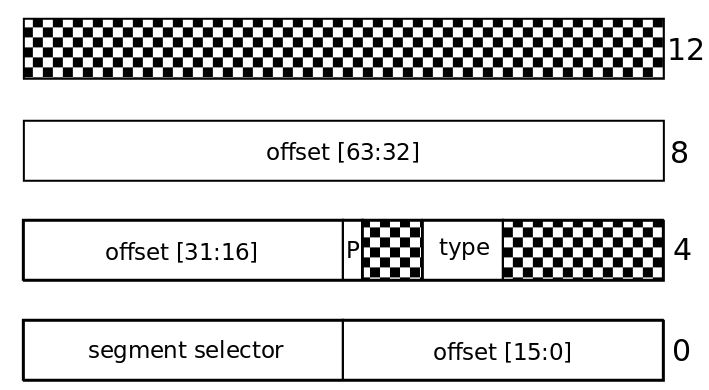
\includegraphics[width=0.5\textwidth]{idt.png}
\end{center}
\begin{itemize}
  \item \emph{offset} - адрес обработчика;
  \item \emph{segment selector} (биты [31:16] в 1-ом слове) - селектор (регистр
  CS);
  \item \emph{P} (Present, бит 15 во 2-ом слове) - должен быть равен 1;
  \item \emph{type} (биты [11:8] во 2-ом слова) - домашнее задание разобраться
  в разнице между Interrup Gate и Trap Gate;
  \item все остальное должно быть равно 0.
\end{itemize}
\end{frame}

\begin{frame}
\frametitle{IDTR}
\begin{center}
  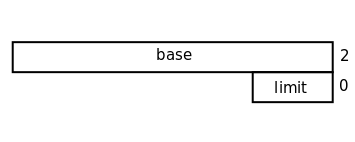
\includegraphics[width=0.6\textwidth]{idt_ptr.png}
\end{center}
\begin{itemize}
  \item Информация о местоположении IDT хранится в специальном регистре (IDTR);
  \item загрузить значение в регистр можно с помощью специальной инструкции
  lidt;
  \begin{itemize}
    \item параметром инструкции является специальный "дескриптор";
    \item \emph{base} - 64-битный адрес IDT в памяти;
    \item \emph{limit} - 16-битный размер IDT в байтах минус единица.
  \end{itemize}
\end{itemize}
\end{frame}

\begin{frame}
\frametitle{Программирование PIC}
\begin{itemize}
  \item Как выбирается какую запись IDT использовать при прерывании?
  \begin{itemize}
    \item вам нужно записать в контроллер на какие записи IDT отображаются
    входы контроллера;
    \item в случае PIC, вам нужно указать на какую запись IDT отображается
    самый первый вход каждого контроллера, все остальные идут по порядку.
  \end{itemize}
  \item Кроме отображения контроллеру прерываний также нужно указать:
  \begin{itemize}
    \item конфигурацию каскада (как Master и Slave соединены);
    \item тип прерывания (edge/level);
    \item и много другого не интересного.
  \end{itemize}
\end{itemize}
\end{frame}

\begin{frame}
\frametitle{Взаимодействие с PIC}
\begin{itemize}
  \item Для общения с PIC используются два 8-ми битных регистра: регистр команд
  и регистр данных;
  \begin{itemize}
    \item в регистр команд записывается действие, которое нужно сделать;
    \item затем в регистр данных записываются данные (сколько и какие именно
    зависит от команды).
  \end{itemize}
  \item Для доступа к регистрам PIC-ов в x86 используется пространство
  ввода/вывода и специальные инструкции работы с ним:
  \begin{itemize}
    \item инструкции называются \emph{in} и \emph{out}, а аргументы порт
    ввода/вывода и данные;
    \item регистр команд Master PIC соответствует порту \emph{0x20}, а регистр
    данных порту \emph{0x21};
    \item Slave PIC использует порты \emph{0xA0} и \emph{0xA1}.
  \end{itemize}
\end{itemize}
\end{frame}

\begin{frame}
\frametitle{Отображение входов PIC}
\begin{itemize}
  \item Чтобы настроить отображение необходимо записать в командный регистр
  значение \emph{0x11} - команда инициализации контроллера;
  \item команда инициализации ожидает три байта данных:
  \begin{itemize}
    \item номер записи IDT, соответвующей самой первому входу контроллера;
    \item параметры каскада:
    \begin{itemize}
      \item для Master PIC - битовую маску входов, к котороым подключены Slave
      PIC-и (в нашем случае это просто \emph{4} - 2-ой бит равен 1, остальные
      0);
      \item для Slave PIC - номер входа Master PIC, к которому он подключен (в
      нашем случае это 2);
    \end{itemize}
    \item прочие неинтересные параметры (в нашем случае нужно записать число
    \emph{1}).
  \end{itemize}
\end{itemize}
\end{frame}

\begin{frame}
\frametitle{Маскировка прерываний}
\begin{itemize}
  \item Иногда полезно запретить доставку определенных прерываний
  (замаскировать)
  \begin{itemize}
    \item до того как драйвер/ОС настроило устройство, прерывания от него лучше
    отключить;
    \item т. е. пре инициализации PIC все прерывания лучше замаскировать.
  \end{itemize}
  \item Для маскировки прерываний в случае PIC используется регистр данных:
  \begin{itemize}
    \item запишите в регистр данных битовую маску прерываний (замаскированным
    соответсвуют 1-цы).
  \end{itemize}
  \item Прерывания можно замаскировать на процессоре
  \begin{itemize}
    \item на x86 это делается инструкцией \emph{cli}, обратная к ней инструкция \emph{sti}.
  \end{itemize}
\end{itemize}
\end{frame}

\begin{frame}
\frametitle{Вызов обработчика прерываний}
\begin{center}
  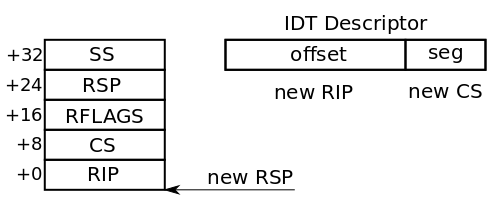
\includegraphics[width=0.6\textwidth]{int_stack.png}
\end{center}
\begin{itemize}
  \item При прерывании процессор сохраняет минимум информации:
  \begin{itemize}
    \item \emph{CS} и \emph{RIP} указывают какой код и с каким уровнем
    привелегий мы прервали;
    \item \emph{RFLAGS} - процессор может менять значение флагового регистра при
    вызове обработчика и сохраняет старое;
    \item \emph{SS} и \emph{RSP} указывают на стек прерваного кода.
  \end{itemize}
\end{itemize}
\end{frame}

\begin{frame}
\frametitle{Обработчик прерывания}
\begin{itemize}
  \item Обработчик прерывания должен сохранить состояние прерванного кода
  \begin{itemize}
    \item как минимум нужно сохрранить регистры общего назначения;
    \item для x86: RAX, RBX, RCX, RDX, RBP, RDI, RSI, R9 - R15.
  \end{itemize}
  \item Обработчик прерывания "должен" вернуть управдление прерванному коду;
  \begin{itemize}
    \item в x86 для этого, \emph{обычно}, используют инструкцию \emph{iretq},
    которая восстанавливает со стека сохраненные регистры CS, SS, RFLAGS, RIP и
    RSP;
    \item т. е. перед исполнением \emph{iretq} стек нужно вернуть в "исходное"
    состояние.
  \end{itemize}
\end{itemize}
\end{frame}

\begin{frame}
\frametitle{End Of Interrupt}
\begin{itemize}
  \item Обработчик прерывания должен нотифицировать контроллер прерывания о
  завершении обработки (послать EOI);
  \begin{itemize}
    \item контроллер прерываний должен знать когда выдать следующий сигнал.
  \end{itemize}
  \item Послать EOI PIC-у можно записав в регистр команд значение специального
  вида:
  \begin{itemize}
    \item \emph{0x60 + irq}, где \emph{irq} - номер входа PIC (от 0 до 7), от
    которого было получено прерывание;
    \item обратите внимание, т. к. PIC-и объединены в каскад, то если прерывание
    пришло на Slave PIC, то EOI нужно посылать сразу и Master и Slave PIC-ам.
  \end{itemize}
\end{itemize}
\end{frame}

\begin{frame}
\frametitle{Исключения}
\begin{itemize}
  \item Во время исполнения команд процессор может обнаружить ошибку:
  \begin{itemize}
    \item попытка исполнить некорректную инструкцию;
    \item недостаточный уровень привелегий, для выполнения действия;
    \item деление на 0;
    \item многое другое...
  \end{itemize}
  \item Такие ситуации называются исключительными и требуют обработки
  \begin{itemize}
    \item x86 сообщает об исключениях в виде прерывания (одного из тех 32
    зарезервированных);
    \item эти прерывания не связаны с контроллерами прерываний и внешними
    устройствами, а являются внутренними для процессора.
  \end{itemize}
\end{itemize}
\end{frame}

\begin{frame}
\frametitle{Критические и некритические ошибки}
\begin{itemize}
  \item В x86 исключения делаться на три категории:
  \begin{itemize}
    \item не критические ошибки (faults) - предполагается, что такие ошибки
    можно исправить и возабновить работу с инструкции приведшей к ошибке (т. е.
    RIP на стеке содержит адрес "плохой" инструкции);
    \item ловушки (traps) - позволяют, условно, отслеживать выполнение некоторых
    инструкций, после обработки исключение управление передается следующей
    инструкции;
    \item критические ошибки (aborts) - с такой ошибкой мало что можно сделать,
    остается только сообщить о ней и "упасть".
  \end{itemize}
\end{itemize}
\end{frame}

\begin{frame}
\frametitle{Особенности обработки исключений в x86}
\begin{center}
  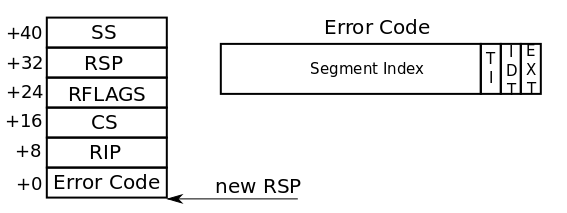
\includegraphics[width=0.6\textwidth]{exc_stack.png}
\end{center}
\begin{itemize}
  \item Для некоторых исключений стек содержит код:
  \begin{itemize}
    \item №8 Double Fault Exception - \emph{Error Code} всегда равен 0;
    \item №10 Invalid TSS Exception;
    \item №11 Segment Not Present;
    \item №12 Stack Fault Exception;
    \item №13 General Protection Exception;
    \item №14 Page-Fault Exception - \emph{Error Code} имеет свой формат;
    \item №17 Alignment Check Exception - \emph{Error Code} 0 или 1.
  \end{itemize}
\end{itemize}
\end{frame}

\begin{frame}
\frametitle{Программные исключения}
\begin{itemize}
  \item Кроме аппаратных прерываний и исключений, есть еще и программные
  прерывания:
  \begin{itemize}
    \item такие прерывания генерируются специальной инструкцией (для x86 это
    \emph{int}, т. е. по сути это trap);
    \item под такие прерывания можно отвести любые незанятые дескрипторы IDT;
    \item так же как и исключения, программные прерывания не связаны с
    контроллером прерываний;
  \end{itemize}
  \item Зачем генерировать исключения программно?
  \begin{itemize}
    \item для вызова привелигерованного кода из непривелигированного;
  \end{itemize}
\end{itemize}
\end{frame}

\begin{frame}
\frametitle{Многопроцессорные системы и прерывания}
\begin{itemize}
  \item Многопроцессорные системы поднимают ряд новых вопросов:
  \begin{itemize}
    \item какой из процессоров должен обрабатывать прерывание?
    \item все ли процессоры эквивалентны для обработки прерываний?
    \item как идентифицировать нужный процессор?
  \end{itemize}
  \item На замену старым PIC-ам в многопроцессорных системах пришли APIC-и
  \begin{itemize}
    \item APIC - Advanced Programmable Interrupt Controller;
    \item например, на ваших домашних компьютерах и ноутбуках используются,
    почти наверняка, используются именно они;
  \end{itemize}
\end{itemize}
\end{frame}

\begin{frame}
\frametitle{APIC}
\begin{columns}
  \begin{column}{0.35\textwidth}
  \begin{center}
    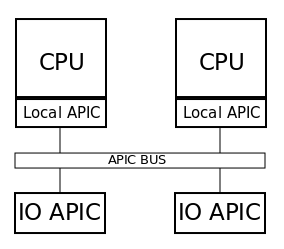
\includegraphics[width=\textwidth]{apic.png}
  \end{center}
  \end{column}
  \begin{column}{0.65\textwidth}
  \begin{itemize}
    \item IO APIC - контроллер, к которому подключаются устройства;
    \begin{itemize}
      \item каждый вход настраивается независимо;
      \item сообщение можно отправить любому Local APIC-у или группе Local
      APIC-ов;
    \end{itemize}
    \item Local APIC - свой у кажого CPU;
    \begin{itemize}
      \item каждый Local APIC имеет свой идентификатор;
      \item Local APIC-и могут обмениваться сообщениями друг с другом;
    \end{itemize}
  \end{itemize}
  \end{column}
\end{columns}
\end{frame}

\begin{frame}
\frametitle{Message Signaled Interrupts}
\begin{itemize}
  \item С обычными прерываниями каждое устройство занимает как минимум один вход
  контроллера прерываний
  \begin{itemize}
    \item несколько устройств могут использовать одну линию, но это может
    создавать трудности;
    \item входы контроллера прерываний нужно "развести" на схеме.
  \end{itemize}
  \item Зачем нам IO APIC и его провода?
  \begin{itemize}
    \item пусть устройства напрямую отправляют сообщения к Local APIC;
    \item реализовать устройство поддерживающее MSI тяжелее, но нет
    необходимости "разделять" прерывания;
    \item MSI обладают меньшими задержками чем обычные прерывания.
  \end{itemize}
\end{itemize}
\end{frame}
